\subsection{Concordance}\label{sec:concord}


The  ECSS-E-ST-40C document or ESA standard for short is shown schematically in \Fig{ecsl2}.
As the report's first author has developed software using a `lite' version of
this standard~\cite{ecss40lite}, it is taken as the reference point. The documents and sections
of documents from the other texts~\cite{hewittexc, Sm17Rati, sommerville10} are
are thus grouped according to the ESA documents, as shown in \Fig{multstruct}.
The other major reference consulted for design of scientific software, namely
Rouson~et~al~\cite{rousonxiaxu}, mainly promotes use of software patterns, albeit 
illustrated by UML diagrams as advocated by refs~\cite{hewittexc, sommerville10}.
\begin{figure}
\centerline{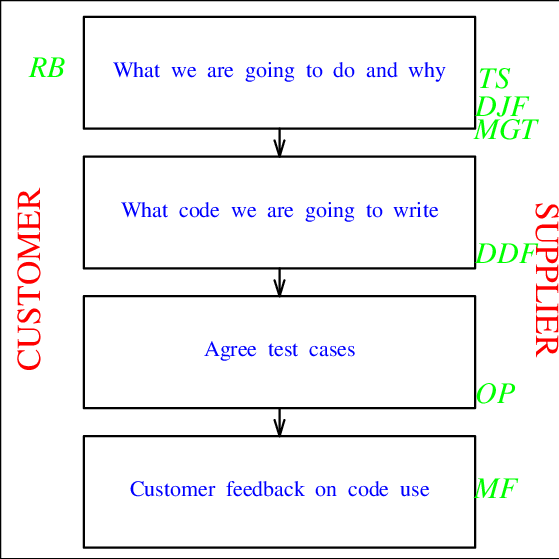
\includegraphics[width=0.7\textwidth]{../png/ecsl2}}
\caption{
Documents according to ECSS-E-ST-40C~\protect{\cite{ecss40exc}},
which is based on a customer-supplier relationship.
The two- and three-letter acronyms indicate document titles as explained
in \Sec{detailedinfo}.
\label{fig:ecsl2}}
\end{figure}
\begin{figure}
\centerline{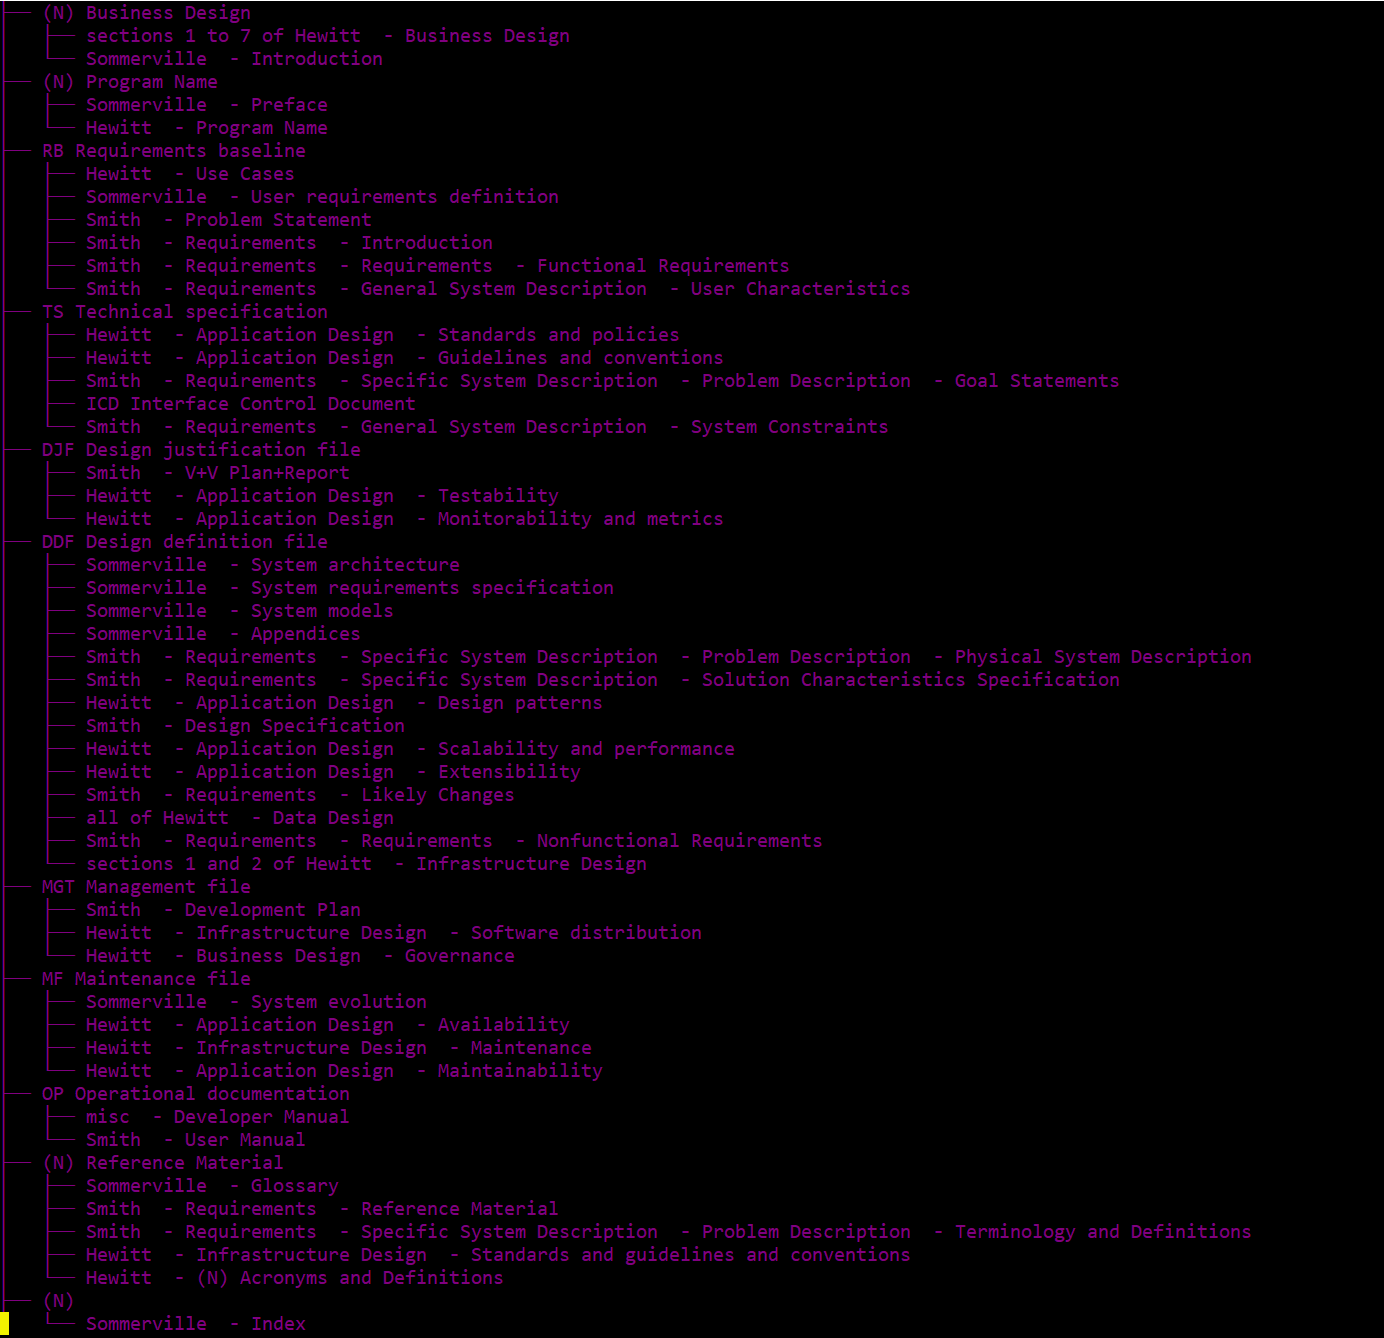
\includegraphics[height=0.9\textheight]{../png/multstruct}}
\caption{Concordance of documents needed during software development,
grouped according to ECSS-E-ST-40C~\protect{\cite{ecss40exc}} - or labelled~`(N)',
texts as follows:
Hewitt ``Semantic Software Design"~\protect{\cite{hewittexc}},
(Spencer)~Smith ``A Rational Document Driven Design Process for Scientific Software"~\protect{\cite{Sm17Rati}},
and Sommerville ``Software Engineering"~\protect{\cite{sommerville10}}.
\label{fig:multstruct}}
\end{figure}

The ESA standard~\cite{ecss40exc} is central because of personal experience that it works, at least in the
``lite" version, seemingly for the reasons that it encourages conversation between the
supplier/paymaster and the developer. These  interactions lead to documentation that
sets out an agreed scope for the software \emph{before} each stage of development,
thus avoiding the project `creep' and on-the-fly redesign that may fatally slow code production.
The Design Justification File (DJF, see~\Sec{DJF}) produced in the process is unique to the ESA documents. Not only does
it prevent untimely customer `what-if's  by setting out and analysing options to a specified time-table,
but constitutes a useful fall-back should the agreed options turn out to be
unworkable when external circumstances change unexpectedly. 

Hewitt~\cite{hewittexc} 
has a good deal of discussion of philosophy which is interesting, amidst
what personal experience indicates should be a very successful methodology
for producing software in a commercial environment, an approach
which is set out both succinctly and comprehensively. His ``Design thinking"
method should be equally useful for encouraging scientific as well as commercial
creativity. This is illustrated in \Fig{hewitt_flowl}, although 
more than one excursion to the tip of the ``$\Lambda$"
might be expected in a research context. It has to be accompanied by a careful
recording of both the good and the bad ideas which emerge.
\begin{figure}
\centerline{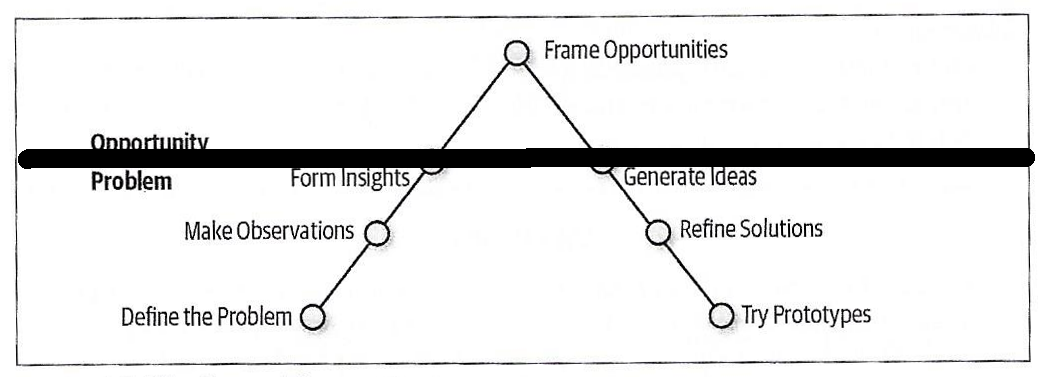
\includegraphics[width=0.9\textwidth]{../png/hewitt_flowl}}
\caption{The Design Thinking process, Figure 4-1 from Hewitt~\protect{\cite{hewittexc}}.
Progression is from left to right: forming insights and generating ideas are both
part of the problem and the opportunity.
\label{fig:hewitt_flowl}}
\end{figure}
Hewitt~\cite{hewittexc} is also very strong on identifying and managing stakeholders beyond the
immediate ambit of the software project. He is understandably less succinct here, letting
it emerge that the average manager is to be treated as someone with a short attention span, principally
focussed on advancing his/her own career (which might include promoting a rival project),
is technically ignorant and likely to demand a PowerPoint justifying any aspect of the project at a moment's notice.
However, in any context, collaborators will appreciate short, to-the-point communications which are clearly presented and well
argued. Hewitt notably also insists on having two reasons for every design decision,
and producing documentation from which it is easy to generate presentations of $5$-$15$~slides.
For commercial reasons, there is also detailed consideration as to how to manage data and
exploit Machine Learning~(ML) tools, and how to 
ensure reliability of both the software and the hardware that it uses, all of which
are germane to the Exascale.
%For commercial reasons, there is as a result of GDPR-type legislation also detailed consideration as to how to manage data, and how 

Spencer Smith~\cite{Sm17Rati}
naturally highlights what documents are needed in the development of \emph{scientific} software.
%contrast Rouson~et~al~\cite{rousonxiaxu} who simply indicate use of UML.
Smith provides reminders of the need to include details such as choice of physical units,
and to plan validation and verification~(V \& V) of results.
Last in the list of sources, Sommerville~\cite{sommerville10} is comprehensive and can be used as
the authority on software terminology in what is still a rapidly expanding subject 
that can give rise to overlapping and even conflicting definitions.

%\input{multstruct_trouted}

\subsection{Detailed Information}\label{sec:detailedinfo}
In this section, the documents labelled~``N'' are introductions  upon the ESA standard
for use in a community project.
Citations in the present section to Hewitt refer specifically to ref~\cite[\S\,5]{hewitt}, to Smith imply ref~\cite[\S\,2.2]{Sm17Rati}
and to Sommerville imply ref~\cite[\S\,4]{sommerville10} unless stated otherwise.
%The concept of self-documenting software is critical??
%Much not needed if usual github/gitlab workflow used. Multimachine not well handled except by docker.
\subsubsection{Program Name PN (N)}\label{sec:PN}
Choice of name for the software is recognised as important, but this section should mainly aim
to give the reader enough information about the purpose of the software
that he/she can decide whether they want to look further.  Hewitt also requires
the equivalent of the approval box for a report, giving names of authors, collaborators and reviewers.
At this point, Hewitt further introduces the RFC2119 subset of the Internet Engineering Task Force~(IETF) keyword~\cite{rfc2119}
for use throughout the document. This usage implies specific meanings for ``MUST", ``MUST NOT", ``REQUIRED", ``SHALL", ``SHALL
NOT", ``SHOULD", ``SHOULD NOT", ``RECOMMENDED",  ``MAY", and ``OPTIONAL" when the words are capitalised.
(It will not be adopted herein.) \\ 
\emph{Think preface to a textbook, plus document approval box.}
\subsubsection{Business Design BD (N)}\label{sec:BD}
This section should aim to make it clear to the reader
why it woud be good to allocate funding for the software development.
From Hewitt's list:
\begin{itemize}
\item Capabilities - what new benefits arise
\item Strategic fit - to UKAEA mission
\item Business drivers - why are we doing this?
\item Assumptions - regarding available funding
\item Constraints - laws and regulations, mention software licensing
\item Risks -  if resources not available
\item Impacts - new processes, training needed
\item Stakeholders - who will win or lose by good or bad outcome
\end{itemize}
\emph{Think introductory chapter of a textbook.}
\subsubsection{Requirements Baseline RB}\label{sec:RB}
The ESA standard RB expresses the customer's requirements, including interface. Sommerville devotes an
entire chapter to requirements engineering, in contrast to Hewitt who
instead recommends `observation' of those working with the software intended for replacement,
and the production of use cases to a detailed template, as follows:
\begin{itemize}
\item Overview
\item Actors
\item Relationship to other use cases
\item Flow including input to output
\item Special requirements
\end{itemize}
The collection of the above use cases then defines the so-called functional requirements,
other requirements are referred to as non-functional. In the scientific case, Spencer Smith
requires specification of the experiment and the assumptions to be used in modelling it.
It is clear since (design) engineers talk of workflows, that Hewitt's approach has much to be recommended
for a mixed engineering/scientific application. \\ 
\emph{This describes the use cases for the software.}
\subsubsection{Technical Specification TS}\label{sec:TS}
The ESA standard TS is the supplier's response to the RB, so provides probably the least useful
ESA document description for a community process.  Material ought nonetheless to be presented
which encompasses the content of the ESA ICD or Interface Control Document. Other material
that would also not be included elsewhere concerns the higher level aspects of Hewitt's Application Design
and Smith's Software Requirements Specification~\cite[\S\,2.2.3]{Sm17Rati}. Hewitt would include
prescription of software standards such as C++17,
and guidelines/conventions such as indicated for Object Fortran in ref~\cite{y2d33}.
Smith would specify what the software needs to compute to compare with experiment.
The need for the code to have good in-line documentation capable of formatting by say \F{Doxygen}~\cite{He21doxy}
will be described here.
\emph{This outlines inputs and outputs of the software, plus set outs principles for code-writing.}
\subsubsection{Design Justification File DJF}\label{sec:DJF}
The ESA standard DJF is generated and reviewed at all stages of the development and review processes.
It contains the documents that describe the trade-offs, design choice justifications, verification plan,
validation plan, validation testing specification,
test procedures, test results, evaluations and any other documentation called for to justify the design of the supplier's product. \\ 
\emph{This describes why the equations, methods and algorithms were chosen, and the testing regime.}
\subsubsection{Design Definition File DDF}\label{sec:DDF}
The ESA standard DDF is a supplier-generated file that
documents the result of the design engineering processes.
The DDF is the primary input to the CDR review process and it contains
all the documents called for by the design engineering requirements. \\ 
\emph{This describes the equations, methods and algorithms to be used in software.}
\subsubsection{Management File MGT}\label{sec:MGT}
The ESA standard MGT is a supplier generated file
that describes the management features of the software project (for instance,
organisational breakdown and responsibilities, work activities breakdown,
selected life cycle, deliveries, milestones and risks).
It also describes governance -  eg.\ PRINCE2~\cite{prince2}. \\ 
\emph{This collates the project plans of all participants.}
\subsubsection{Maintenance File MF}\label{sec:MF}
The MF is a maintainer generated file
that describes the planning and status of the maintenance, migration and retirement activities. \\ 
\emph{This is basically unnecessary given one of the common repository-based projects.}
\subsubsection{Operational Documentation OP}\label{sec:OP}
In the ESA standard OP, the user's experience of the software feeds back into the instructions
as to how to use the software. \\ 
\emph{This includes the user manual, the developer manual and describes output of test cases.}
\subsubsection{Reference Material REF (N)}\label{sec:REF}
In a web-based system, this material can be presented stand-alone to avoid duplication throughout
many different documents. It should provide an ontology for the project, by which it is meant
a glossary of terminology used, meanings of acronyms and an index of mathematical notation.
%special definitions for the project
\subsubsection{Index IND (N)}\label{sec:IND}
The construction of an index is recommended by Sommerville, and although an alphabetic index
is made redundant by web search engines, it might be helpful to have an index of diagrams and figures.

\subsection{Production of .html}\label{sec:toweb}
%Mentioned in the Introduction~\Sec{intro},
It has become recently very popular to construct web-based code documentation using `Read the
Docs'~\cite{readthedocswebsite}, which is open-source software that indeed
produces a very attractive website, see eg.\ the plasmapy~\cite{plasmapywebsite} website.
The problem is the need to use reStructuredText or Markdown
formats to input to  `Read the Docs'. For many people, both formats represent yet more markup languages to learn, and
although many know Markdown, it has many slightly incompatible variants.
Similar criticism applies to the use of \F{Doxygen} for producing documentation other
than in-line at a relatively low level.
Fortunately the open-source \F{pandoc} project~\cite{pandocwebsite}  has in the last
few years (Version~2.5 from~2018, or later) developed to the point where it can turn relatively complex \LaTeX\ 
documents into .html for display using web browsers.  \F{pandoc} also tightly defines a variant
of Markdown that it would be good to employ as a standard, since \F{pandoc} can then
use files conforming to this standard to produce output in many different
formats.

As with  many open source projects, a certain amount of experimentation is needed to 
locate suitable options for \F{pandoc}, especially as it is under active development at the time
of writing. The following bash shell script produces readable .html from a report
including all the \verb-\-\T{input} files
with Version~2.5, current on Ubuntu as of March~2021:
\begin{verbatim}
pandoc $1.tex --metadata pagetitle=$1 --toc  \
--number-sections \
--bibliography ../bib/exc.bib \
--bibliography ../bib/reac.bib \
-s --mathml --default-image-extension=png -o $1.html
\end{verbatim}
The \T{--verbose} option is useful as otherwise only terse error messages appear.
\F{pandoc} is strict in its interpretation of \LaTeX, so that eg.\ \verb-\-\T{mathbf }
and \verb-\-\T{texttt} need to be used instead of \verb-\-\T{bf} and \verb-\-\T{tt},
and extended character sets may cause \F{pandoc} to fail.
\verb-\-\T{rotatebox} and \verb-\-\T{protect} are not recognised and should be stripped from 
the .tex file using \I{sed} before processing.

For the power shell with \F{pandoc}~Version 2.12 dated~2021, the following produces
readable .html from the report:
\begin{verbatim}
pandoc rp3.tex --metadata pagetitle=rp3 --toc `
--number-sections `
--bibliography ../bib/exc.bib `
--bibliography ../bib/reac.bib `
--bibliography ../bib/waynes.bib `
--bibliography ../bib/new.bib `
--bibliography ../bib/active.bib `
--bibliography ../bib/mc.bib `
-s --citeproc --mathml --default-image-extension=png -o rp3.html
\end{verbatim}
However the \T{--mathjax} option needs to replace \T{--mathml} for mathematics
to display correctly in the Microsoft Edge browser.
%#--bibliography ../bib/exc.bib \
%#--bibliography ../bib/new.bib \
%#--bibliography ../bib/waynes.bib \
%#--bibliography ../bib/misc.bib \
%#--bibliography ../bib/warv.bib \
%#--bibliography ../bib/neuts.bib \
%#--bibliography ../bib/reac.bib \
%#--bibliography ../bib/active.bib \
%#--bibliography ../bib/dg1srt.bib \

Although there are still significant issues regarding the .html produced, \F{PANDOC}
has demonstrated an ability to format equations and produce bibliographies that
suggests that it could become a powerful tool in the production of documentation
to underpin the \nep\ software development. Consideration should be given to making
resource available to ensure the tool provides all necessary facilities in an easy-to-use
wrapper.
